\documentclass[fontset=windows]{article}
\usepackage[margin=1in]{geometry}%设置边距,符合Word设定
\usepackage[UTF8]{ctex}
\usepackage{setspace}
\usepackage{amsmath}
\usepackage{amssymb}
\numberwithin{figure}{section}
\usepackage{array}
\usepackage{lipsum}
\usepackage{float}
\usepackage{graphicx}%插入图片
\usepackage[dvipsnames]{xcolor}
\usepackage{authblk}
\usepackage{listings,matlab-prettifier}
\lstset{
	language=Matlab, % 设置代码语言为Matlab
    basicstyle=\ttfamily, % 设置字体为等宽字体
    numbers=left, % 行号在左边显示
    numberstyle=\tiny, % 设置行号字体大小
    stepnumber=1, % 行号递增步长
    numbersep=5pt, % 行号到代码的距离
    backgroundcolor=\color{gray!10}, % 设置代码的背景颜色
    showspaces=false,
    showstringspaces=false,
    showtabs=false,
    frame=single, % 设置代码框
    rulecolor=\color{black},
    tabsize=2,
    breaklines=true,
    breakatwhitespace=true,
    title=\lstname,
	keywordstyle=\bfseries\color{NavyBlue},
	morekeywords={var,};
	emphstyle=\bfseries\color{Rhodamine}, % 强调词样式设置
    commentstyle=\itshape\color{black!50!white}, % 设置注释样式,斜体,浅灰色
    stringstyle=\bfseries\color{PineGreen!90!black}, % 设置字符串样式
	columns=flexible,}
\graphicspath{{Figures4/}}%文章所用图片在当前目录下的 Figures目录

\usepackage{hyperref} % 对目录生成链接,注:该宏包可能与其他宏包冲突,故放在所有引用的宏包之后
\hypersetup{colorlinks = true,  % 将链接文字带颜色
	linkcolor=black, % 将链接文字黑色
	bookmarksopen = true, % 展开书签
	bookmarksnumbered = true, % 书签带章节编号
	} % 作者
\bibliographystyle{plain}% 参考文献引用格式

\renewcommand{\contentsname}{\centerline{目录}} %经过设置word格式后,将目录标题居中

\title{\heiti\zihao{2} 《统计信号处理》第四教学单元研讨题}
\author{杨 鼎,韦可雷,高司博,高涵博}
\date{}

\begin{document}
\maketitle
\thispagestyle{empty}

%\begin{abstract}
%	\lipsum[2]
%\end{abstract}

%\tableofcontents
%\setcounter{page}{0}
%\newpage

\section{第一题}
卡尔曼滤波器中,过去的观测是如何对当前的状态估计起作用的?你认为影响当前状态估计性能的因素有哪些?
能否在滤波过程开始之前就确定滤波的性能?为什么?卡尔曼滤波中,哪些步骤需要再线计算?哪些步骤可以离线计算?
能否在滤波过程开始之前就确定滤波的性能?为什么?


\subsection*{(1)卡尔曼滤波器中,过去的观测是如何对当前的状态估计起作用的?}

在卡尔曼滤波中,可以由信号模型、观测模型中确定性的部分,
利用过去的观测数据进行一步预测、观测预测,滤波利用预测和卡尔曼增益加以修正。

\subsection*{(2)你认为影响当前状态估计性能的因素有哪些?}

影响当前状态估计的性能的因素有扰动噪声、观测噪声,状态转移矩阵和观测矩阵。

\subsection*{(3)能否在滤波过程开始之前就确定滤波的性能?为什么?}

能在开始前确定滤波性能。因为卡尔曼增益和滤波方差阵与当前测量值无关,可以提前获得,即可得知滤波性能。

\subsection*{(4)卡尔曼滤波中,哪些步骤需要再线计算?哪些步骤可以离线计算?}

卡尔曼增益和滤波误差方差阵和观测数据无关,可以离线计算。
预测误差方差阵和滤波需要在线计算

\section{第二题}
标量状态-标量观测卡尔曼滤波器模型
\begin{align*}
    s[n] & =as[n-1]+w[n] \\
    z[n] & =s[n]+v[n]
\end{align*}
设\(a=0.9.\sigma_w^2=1,\mu_s=0,\sigma_s^2=1,E(v[n])^2=\sigma_n^2\),如果:

(1)\(\sigma_n^2=0.9^n\);

(2)\(\sigma_n^2=1.1^n\);

求卡尔曼增益、最小MSE,并利用计算机进行仿真,给出滤波误差曲线。

对于标量状态-标量观测卡尔曼滤波器模型,卡尔曼滤波器各个步骤的表达式为:

预测:
\begin{align*}
    \hat{s}[n|n-1] =a\hat{s}[n-1|n-1]
\end{align*}
最小预测MSE:
\begin{align*}
    M[n|n-1] & =a^2M[n-1|n-1]+\sigma_w^2 \\
             & =a^2M[n-1|n-1]+1
\end{align*}
卡尔曼增益:
\begin{align*}
    K[n]         =\frac{M[n|n-1]}{\sigma_n^2+M[n|n-1]}
\end{align*}
修正:
\begin{align*}
    \hat{s}[n|n] =\hat{s}[n|n-1]+K[n](x[n]-\hat{s}[n|n-1])
\end{align*}
最小MSE:
\begin{align*}
    M[n|n]       =(1-K[n])M[n|n-1]
\end{align*}

\subsection*{(1)当\(\sigma_n^2=0.9^n\)时,求卡尔曼增益、最小MSE,并利用计算机进行仿真,给出滤波误差曲线。}

当\(\sigma_n^2=0.9^n\)时,最小MSE为
\begin{align*}
    M[n|n]=(1-K[n])M[n|n-1]=\frac{0.9^nM[n|n-1]}{0.9^n+M[n|n-1]}
    \overset{n\to +\infty}{\to} 0
\end{align*}

卡尔曼增益为
\begin{align*}
    K[n] & =\frac{M[n|n-1]}{\sigma_n^2+M[n|n-1]} \\
         & =\frac{M[n|n-1]}{0.9^n+M[n|n-1]}      \\
         & = \frac{1}{1+\frac{0.9^n}{M[n|n-1]}}  \\
\end{align*}
当卡尔曼滤波器收敛时,最小MSE将趋近于观测误差\(\sigma^2_n=0.9^n\),
因此,当\(n\to \infty\)时,\(M[n|n-1]\)与\(0.9^n\)收敛速度相近,K[n]将收敛于常数。

\begin{figure}[H]
    \centering
    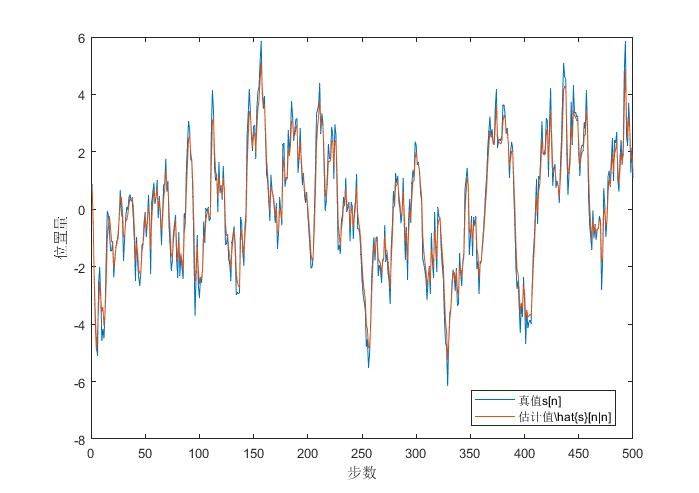
\includegraphics[scale=0.5]{2_1.jpg}
    \caption{状态s[n]与估计量\(\hat{s}\)[n|n]的曲线比较}
    \label{2.1}
\end{figure}

\begin{figure}[H]
    \centering
    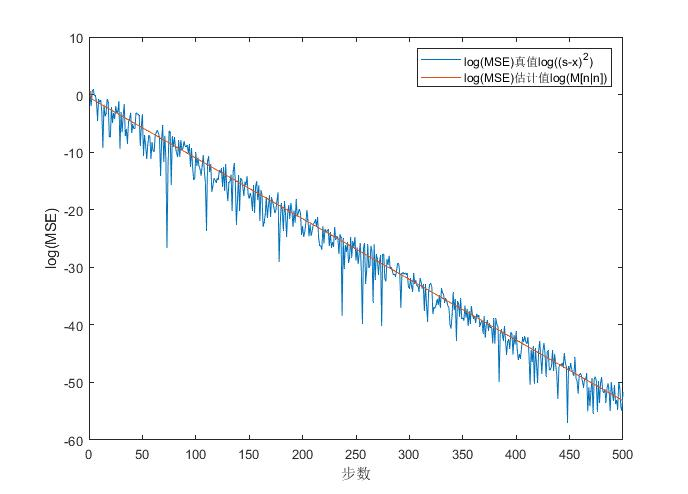
\includegraphics[scale=0.5]{2_2.jpg}
    \caption{滤波误差log(MSE)与卡尔曼滤波最小MSE的对数log(M[n|n])的曲线比较}
    \label{2.2}
\end{figure}

图2.1和图2.2分别显示了步数\(n\to 500\)过程中,当\(\sigma_n^2=0.9^n\)时,卡尔曼滤波状态量和误差的变化曲线比较。
从图2.1中可以看出卡尔曼滤波估计量\(\hat{s}[n|n]\)与状态量s[n]变化不大,
说明卡尔曼滤波能够跟上观测噪声的变化,图2.2也证明了这一点。
图2.2显示了滤波误差的对数log(MSE)与卡尔曼滤波误差估计最小MSE的对数log(M[n|n]),随n增加的变化曲线。
当\(n\to 500\)时,\(MSE\to 0\),说明卡尔曼滤波最终达到收敛。


\subsection*{(2)当\(\sigma_n^2=1.1^n\)时,求卡尔曼增益、最小MSE,并利用计算机进行仿真,给出滤波误差曲线。}

当\(\sigma_n^2=1.1^n\)时,最小MSE为
\begin{align*}
    M[n|n]=(1-K[n])M[n|n-1]=\frac{1.1^nM[n|n-1]}{1.1^n+M[n|n-1]}
    \overset{n\to +\infty}{\to} +\infty
\end{align*}

卡尔曼增益为
\begin{align*}
    K[n] & =\frac{M[n|n-1]}{\sigma_n^2+M[n|n-1]} \\
         & =\frac{M[n|n-1]}{1.1^n+M[n|n-1]}      \\
         & = \frac{1}{1+\frac{1.1^n}{M[n|n-1]}}  \\
\end{align*}

与第一问类似,当\(n\to +\infty\)时,K[n]将收敛于常数。

\begin{figure}[H]
    \centering
    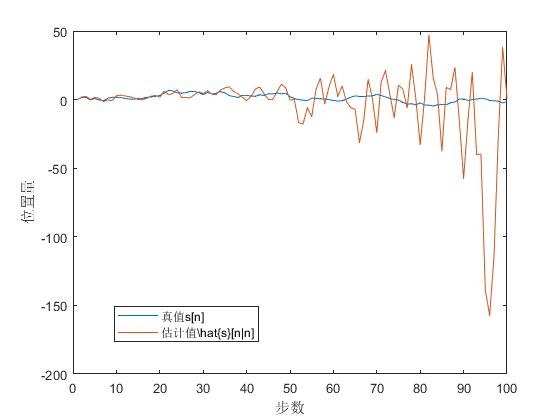
\includegraphics[scale=0.5]{2_3.jpg}
    \caption{状态s[n]与估计量\(\hat{s}\)[n|n]的曲线比较}
    \label{2.3}
\end{figure}

\begin{figure}[H]
    \centering
    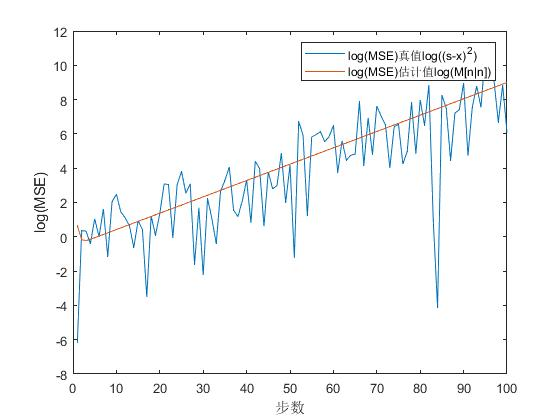
\includegraphics[scale=0.5]{2_4.jpg}
    \caption{状态s[n]与估计量\(\hat{s}\)[n|n]的曲线比较}
    \label{2.4}
\end{figure}

图2.3和图2.4分别显示了步数\(n\to 100\)过程中,当\(\sigma_n^2=1.1^n\)时,卡尔曼滤波状态量和误差的变化曲线比较。
从图2.3中可以看出卡尔曼滤波逐渐发散,不能逼近于真实值,这时由于卡尔曼滤波方程中最小MSE\(M[n|n]\)趋向于发散,
图2.4也验证了这一点。

\section{第三题}
某目标在二维平面x-y上运动,两个方向的速度可以用AR模型描述:\(v_x[k]=\rho v_x[k-1]+n_x[k]
v_y[k]=\rho v_y[k-1]+n_y[k]\)。由于目标的速度是变化的,将k-1时刻到k时刻的目标运动近似为匀加速运动,
此时目标位置变化可以用下式描述:
\begin{align*}
    x[k] & =x[k-1]+\frac{v_x[k-1]+v_x[k]}{2}\cdot T \\
    y[k] & =y[k-1]+\frac{v_y[k-1]+v_y[k]}{2}\cdot T
\end{align*}

试写出目标位置滤波所需的状态方程、观测方程和卡尔曼滤波各个步骤的表达式。

\subsection*{(1)状态方程}

设状态矢量\(\mathbf{a}[k]=\begin{bmatrix}
    x[k] & v_x[k] & y[k] & v_y[k]
\end{bmatrix}^T\),由于

\begin{align*}
    x[k]   & =x[k-1]+\frac{v_x[k-1]+v_x[k-1]}{2}T             \\
           & =\frac{x[k-1]+\rho v_x[k-1]+n_x[k]}{2}T          \\
    v_x[k] & =\rho v_x[k-1]+n_x[k]                            \\
    y[k]   & =y[k-1]+\frac{v_y[k-1]+v_y[k]}{2}T               \\
           & =y[k-1]+\frac{v_y[k-1]+\rho v_y[k-1]+n_y[k]}{2}T \\
    v_y[k] & =\rho v_y[k-1]+n_y[k]
\end{align*}

状态方程\(\mathbf{a}[k]=\boldsymbol{\Phi}\mathbf{a}[k-1]+\mathbf{\Gamma n}[k]\),其中
\begin{align*}
    \boldsymbol{\Phi}=
    \begin{bmatrix}
        1 & \frac{T}{2}(1+\rho) & 0 & 0                   \\
        0 & \rho                & 0 & 0                   \\
        0 & 0                   & 1 & \frac{T}{2}(1+\rho) \\
        0 & 0                   & 0 & \rho
    \end{bmatrix},
    \mathbf{n}[k]=
    \begin{bmatrix}
        n_x[k] \\
        n_y[k]
    \end{bmatrix},
    \boldsymbol{\Gamma}[k]=
    \begin{bmatrix}
        \frac{T}{2} & 0           \\
        1           & 0           \\
        0           & \frac{T}{2} \\
        0           & 1
    \end{bmatrix}
\end{align*}

假定风速修正等在任何地方以同样的幅度出现,给\(n_x[k]\)和\(n_y[k]\)赋予相同的方差,并且假定他们都是独立的,
则\(n[k]\)为零均值白噪声,方差阵
\begin{align*}
    \mathbf{Q}=E(\mathbf{n}[k]^T\mathbf{n}[k])
    =\begin{bmatrix}
        \sigma^2_n & 0          \\
        0          & \sigma^2_n
    \end{bmatrix}=\sigma^2_n \mathbf{I}
\end{align*}

\subsection*{(2)观测模型}

\begin{align*}
    z_x[k] & =x[k]+w_x[k] \\
    z_y[k] & =y[k]+w_y[k]
\end{align*}
令
\begin{align*}
    \mathbf{z}[k]=
    \begin{bmatrix}
        z_x[k] \\
        z_y[k]
    \end{bmatrix},
    \mathbf{w}[k]=
    \begin{bmatrix}
        w_x[k] \\
        w_y[k]
    \end{bmatrix},
    \mathbf{H}=
    \begin{bmatrix}
        1 & 0 & 0 & 0 \\
        0 & 0 & 1 & 0
    \end{bmatrix}
\end{align*}

则观测方程可以表示为
\begin{align}
    \mathbf{z}[k]=\mathbf{Ha}[k]+\mathbf{w}[k]
\end{align}

同理,令不同方向的观测误差也是独立的,且方差相同,则\(\mathbf{w}[k]\)也为零均值白噪声,方差阵
\(\mathbf{R}=E(\mathbf{w}[k]^T\mathbf{w}[k])=\begin{bmatrix}
    \sigma^2 & 0        \\
    0        & \sigma^2
\end{bmatrix}=\sigma^2\mathbf{I}\)

\subsection*{(3)卡尔曼滤波各个步骤表达式}

预测:
\begin{align*}
    \hat{\mathbf{a}}[k|k-1]=\boldsymbol{\Phi}\hat{\mathbf{a}}[k-1|k-1]
\end{align*}

预测误差方差阵:
\begin{align*}
    \mathbf{P}_{\hat{\mathbf{a}}}[k|k-1]=\boldsymbol{\Phi}\mathbf{P}_{\hat{\mathbf{a}}}[k-1|k-1]
    \boldsymbol{\Phi}^T+\sigma^2_n \boldsymbol{\Gamma \Gamma}^T
\end{align*}

增益:
\begin{align*}
    \mathbf{K}[k]=\mathbf{P}_{\hat{a}}[k|k-1]\mathbf{H}^T
    (\mathbf{H P}_{\hat{\mathbf{a}}}[k|k-1]\mathbf{H}^T+\sigma^2\mathbf{I})^{-1}
\end{align*}

滤波:
\begin{align*}
    \hat{\mathbf{a}}[k|k]=\hat{\mathbf{a}}[k|k-1]+\mathbf{K}[k]
    (\mathbf{z}[k]-\mathbf{H} \hat{\mathbf{a}}[k|k-1])
\end{align*}

滤波误差方差阵:
\begin{align*}
    \mathbf{P}_{\hat{\mathbf{a}}}[k|k]=
    (\mathbf{I}-\mathbf{K}[k]\mathbf{H})\mathbf{P}_{\hat{\mathbf{a}}}[k|k-1]
\end{align*}

\section{第四题}
\subsection*{结合清华大学出版社的《统计信号处理》(第二版)9.6.2节中雷达无人机跟踪场景,
    采用卡尔曼滤波实现无人机位置和速度的估计。}

\begin{figure}[H]
    \centering
    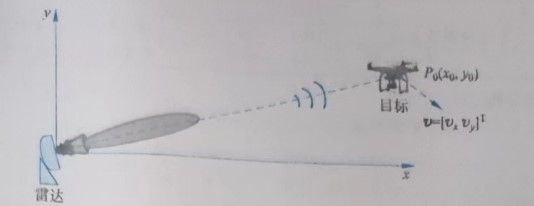
\includegraphics[scale=0.8]{4_1.jpg}
    \caption{无人机目标跟踪示意图}
    \label{4.1}
\end{figure}

无人机目标跟踪如图4.1所示。只考虑平面运动。设无人机从初始位置\(P_0(x_0,y_0)\)开始,
以恒定的速度\(\mathbf{v}=[v_x,v_y]^T\)做匀速直线运动,时刻的位置为\(\mathbf{x}(t)=[x(t),y(t)]^T\)。
雷达位于坐标原点,假定雷达可以测量t时刻目标的斜距\(r(t)\)和方位角\(\theta(T)\),且测距、测角误差相互独立。
考虑到斜距和方位角均为目标位置的非线性函数,为了方便可利用
\begin{align}
    \left\{
    \begin{matrix}
        x(t) & =r(t)\cos\theta(t) \\
        y(t) & =r(t)\sin\theta(t)
    \end{matrix}
    \right.
\end{align}

获得等效的直角坐标模型,测量方程可以写为
\begin{align*}
    \mathbf{z}(t_n)=\mathbf{x_n}+\boldsymbol{\epsilon}(t_n)
\end{align*}
其中\(\mathbf{x}(t_n)=[x(t_n),y(t_n)]^T\),表示\(t_n\)时刻目标在直角坐标系内的位置矢量,
\(\boldsymbol{\epsilon}(t_n)=[\epsilon_x (t_n),\epsilon_y (t_n)]^T\)为等效观测噪声,
T为测量数据的采样间隔,假定等效观测噪声为不相关的高斯噪声通常斜距和方位角测量误差可用独立正态随机变量描述,
由于式1为非线性函数,因此直角坐标系下等效观测的x、y分量之间存在相关性。事实上,由式1可知
\begin{align}
    \left\{
    \begin{matrix}
        \Delta x & \approx \Delta r \cos \theta-r \sin\theta \Delta \theta \\
        \Delta y & \approx \Delta r \sin\theta+r \cos\theta \Delta \theta
    \end{matrix}
    \right.
\end{align}
其中,\(E(\Delta r)\approx 0,E(\Delta \theta)\approx 0,E((\Delta r)^2)\approx \sigma^2_r,
E((\Delta \theta)^2)\approx 0\)。

考虑信号模型
\begin{align*}
    \mathbf{x}[k+1]=\boldsymbol{\Phi}\mathbf{x}[k]+\boldsymbol{\Gamma}\mathbf{n}[k]
\end{align*}
其中
\begin{align*}
    \mathbf{x}[k]=
    \begin{bmatrix}
        x[k]       \\
        \dot{x}[k] \\
        y[k]       \\
        \dot{y}[k]
    \end{bmatrix},
    \mathbf{n}[k]=
    \begin{bmatrix}
        a_x[k] \\
        a_y[k]
    \end{bmatrix},
    \boldsymbol{\Phi}=
    \begin{bmatrix}
        1 & T & 0 & 0 \\
        0 & 1 & 0 & 0 \\
        0 & 0 & 1 & T \\
        0 & 0 & 0 & 1
    \end{bmatrix},
    \boldsymbol{\Gamma}=
    \begin{bmatrix}
        T^2/2 & 0     \\
        T     & 0     \\
        0     & T^2/2 \\
        0     & T
    \end{bmatrix}
\end{align*}
\(n[k]\)为零均值白噪声,方差阵为
\begin{align*}
    \mathbf{Q}=E\left(\mathbf{n}[k]\mathbf{n}^T[k]\right)
    =\begin{bmatrix}
        \sigma^2_a & 0          \\
        0          & \sigma^2_a
    \end{bmatrix}=\sigma^2_a\mathbf{I}
\end{align*}

令
\begin{align*}
    \mathbf{z}[k]=
    \begin{bmatrix}
        z_x[k] \\
        z_y[k]
    \end{bmatrix},
    \mathbf{w}[k]=
    \begin{bmatrix}
        w_x[k] \\
        w_y[k]
    \end{bmatrix},
    \mathbf{H}=
    \begin{bmatrix}
        1 & 0 & 0 & 0 \\
        0 & 0 & 1 & 0
    \end{bmatrix}
\end{align*}

测量方程可以表示为:
\begin{align*}
    \mathbf{z}[k]=\mathbf{Hx}[k]+\mathbf{w}[k]
\end{align*}
其中\(w[k]\)的方程阵为
\begin{align*}
    \mathbf{R}=
    \begin{bmatrix}
        \sigma^2_r\cos^2\theta+r^2\sigma^2_{\theta}\sin^2\theta
         & (\sigma^2_r-r^2\sigma^2_{\theta}\sin\theta\cos\theta)   \\
        (\sigma^2_r-r^2\sigma^2_{\theta}\sin\theta\cos\theta)
         & \sigma^2_r\sin^2\theta+r^2\sigma^2_{\theta}\cos^2\theta
    \end{bmatrix}
\end{align*}

因此卡尔曼滤波算法如下:

预测:
\begin{align*}
    \hat{\mathbf{x}}[k|k-1]=\boldsymbol{\Phi}[k,k-1]\hat{\mathbf{x}}[k|k-1]
\end{align*}
预测误差方差阵:
\begin{align*}
    \mathbf{P}_{\hat{\mathbf{x}}}=
    \boldsymbol{\Phi}[k,k-1]\mathbf{P}_{\hat{\mathbf{x}}}[k-1|k-1]
    \boldsymbol{\Phi}^T[k,k-1]+\boldsymbol{\Gamma}[k-1]\mathbf{Q}[k-1]\boldsymbol{\Gamma}^T[k-1]
\end{align*}
增益:
\begin{align*}
    \mathbf{K}[k]=\mathbf{P}_{\hat{\mathbf{x}}}[k|k-1]\mathbf{H}^T[k]
    (\mathbf{H}[k]\mathbf{P}_{\hat{\mathbf{x}}}[k|k-1]\mathbf{H}^T[k]+\mathbf{R}[k])^{-1}
\end{align*}
滤波:
\begin{align*}
    \hat{\mathbf{x}}[k|k]=\hat{\mathbf{x}}[k|k-1]+\mathbf{K}[k]
    (\mathbf{z}[k]-\mathbf{H}[k]\hat{\mathbf{x}[k|k-1]})
\end{align*}
滤波误差方差阵:
\begin{align*}
    \mathbf{P}_{\hat{\mathbf{x}}}[k|k]=(\mathbf{I}-\mathbf{K}[k]\mathbf{H}[k])
    \mathbf{P}_{\hat{\mathbf{x}}}[k|k-1]
\end{align*}
需要注意的是,此时的R是一个跟观测斜矩和方位角有关的量,因此每次卡尔曼迭代的过程中都需要更新R。

用两点法进行起始:
\begin{align*}
    \hat{\mathbf{x}}=
    \begin{bmatrix}
        z_x[2]                  \\
        \frac{z_x[2]-z_x[1]}{T} \\
        z_y[2]                  \\
        \frac{z_y[2]-z_y[1]}{T}
    \end{bmatrix},
    \mathbf{P}_{\hat{\mathbf{x}}}[2|2]=
    \begin{bmatrix}
        p_{11} & p_{12} & 0      & 0      \\
        p_{21} & p_{22} & 0      & 0      \\
        0      & 0      & p_{33} & p_{34} \\
        0      & 0      & p_{43} & p_{44}
    \end{bmatrix}
\end{align*}

因为观测误差的\(w_x[k],w_y[k]\)之间是相关的,因此起始滤波误差方差阵计算起来较为麻烦,
但是因为起始值的选取只影响卡尔曼滤波的前几个结果,因此先默认\(w_x[k],w_y[k]\)之间是不相关的,此时:
\begin{align*}
    p_{11} & =\sigma^2_1                      \\
    p_{12} & =\frac{\sigma^2_1}{T}            \\
    p_{22} & =T^2\sigma^2_a/4+2\sigma^2_1/T   \\
    p_{33} & =\sigma^2_2                      \\
    p_{34} & =\frac{\sigma^2_2}{T}            \\
    p_{44} & =T^2\sigma^2_a/4+2\sigma^2_2/T^2
\end{align*}
其中,
\begin{align*}
    \sigma_1^2 & =\sigma^2_r\cos^2\theta+r^2\sigma^2_{\theta}\sin^2\theta \\
    \sigma^2_2 & =\sigma^2_r\sin^2\theta+r^2\sigma^2_{\theta}\cos^2\theta
\end{align*}

采用该方法进行100次的蒙特卡洛仿真,设置目标初始坐标为(1000m,4000m),目标速度为(10m/s,-8m/s)测距误差标准差2m,
测角误差标准差为0.56°,采样间隔0.25s,单次仿真采样总时长为100s,扰动加速度标准差为0.001m/s²,仿真结果如下:

轨迹之间的对比图以及速度对比图如图4.2和图4.3所示:

\begin{figure}[H]
    \centering
    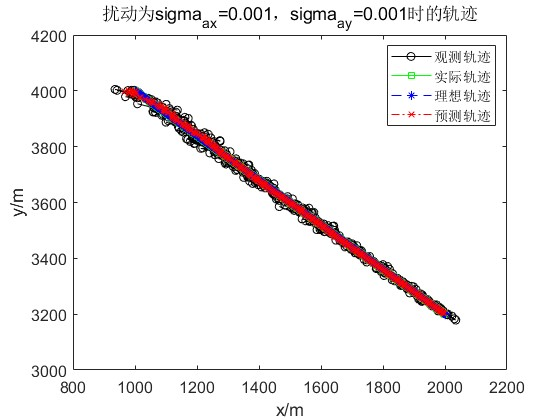
\includegraphics[scale=0.8]{4_2.jpg}
    \caption{扰动为\(\sigma_{ax}=0.001,\sigma_{ay}=0.001\)时的轨迹}
    \label{4.2}
\end{figure}

\begin{figure}[H]
    \centering
    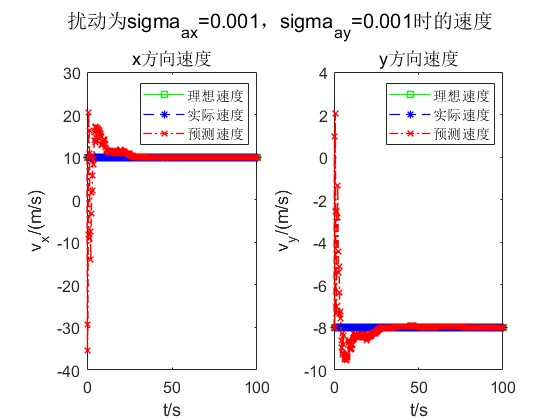
\includegraphics[scale=0.8]{4_3.jpg}
    \caption{扰动为\(\sigma_{ax}=0.001,\sigma_{ay}=0.001\)时的速度}
    \label{4.3}
\end{figure}

由图可知通过滤波可以平滑观测曲线,使其更加接近实际轨迹,同时初始值的选取只会影响到前几个预测值。
单次观测的滤波误差结果如图4.4所示:

\begin{figure}[H]
    \centering
    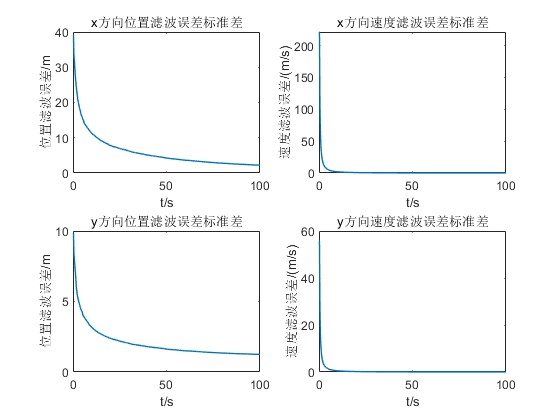
\includegraphics[scale=0.9]{4_4.jpg}
    \caption{单次观测的滤波误差}
    \label{4.4}
\end{figure}

\bibliography{books}
\end{document}